\documentclass[../main.tex]{subfiles}

\graphicspath{{\subfix{../images/}}}

\begin{document}

\section{Part 1 - Modelling and Simulations}

\subsection{Task 1.1}

Draw the equivalent circuit model to be used to simulate the crosstalk in each of the 3 cases.

\vspace{10pt}
The model must include the driver circuit (linear model), package parasitics (simple model), transmission lines, and probe points, and receiver circuit (linear model).

\solution

To model the driver, receiver and all package parasitics we will use an IBIS model for the 74ALVC244 buffer chip. We start by describing how the IBIS specification can be used to model the buffer. 

\subsubsection{Buffer Output Model}

Consider the generic three-state output buffer shown in Figure \ref{fig:ibis-buffer}.

\begin{figure}[h]
    \centering
    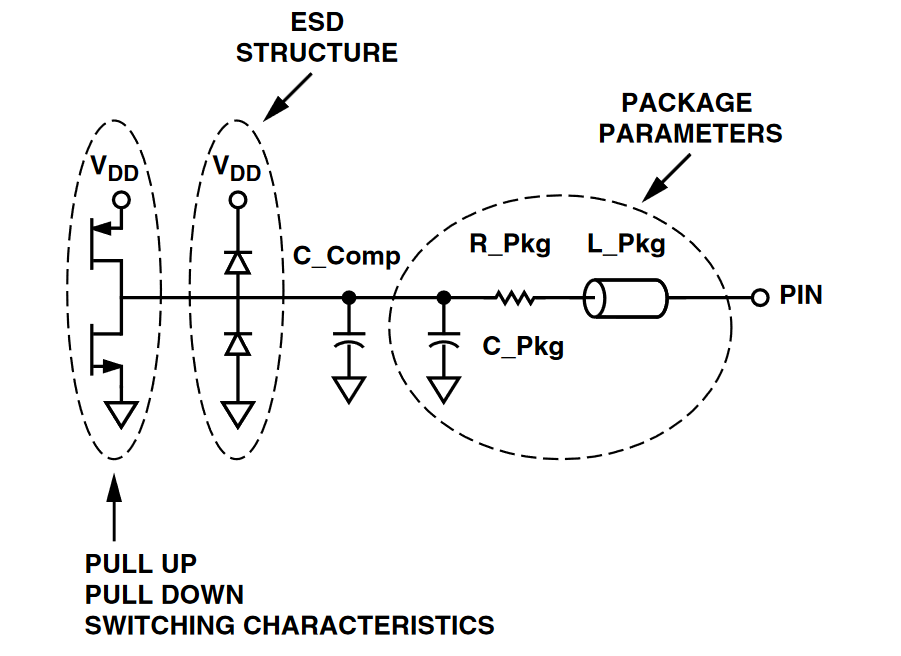
\includegraphics[width=0.5\textwidth]{three-state-ibis.png}
    \caption{Three-state output buffer\footcite{ibis}.}
    \label{fig:ibis-buffer}
\end{figure}

In our case we will model the output of the CMOS devices as a voltage source with a series resistance. The capacitor $C_{comp}$ will be used to model the ramp rate of the falling and rising waveforms. $C_{comp}$ is the silicon die capacitance, and does \textbf{not} include the package parasitics. $R_{pkg}, C_{pkg}, L_{pkg}$ are the electrical characteristics for each pin-to-buffer connection. They are the lumped elements of the overall package\footcite{ibis}.

\vspace{10pt}
The linear model of the driver circuit is shown in Figure \ref{fig:driver-package}. $V_1, R_1. C_1$ constitute the driver model, and $R_2, C_2, L_2$ are the QFN package parasitics.

\begin{figure}[h]
    \centering
    \fbox{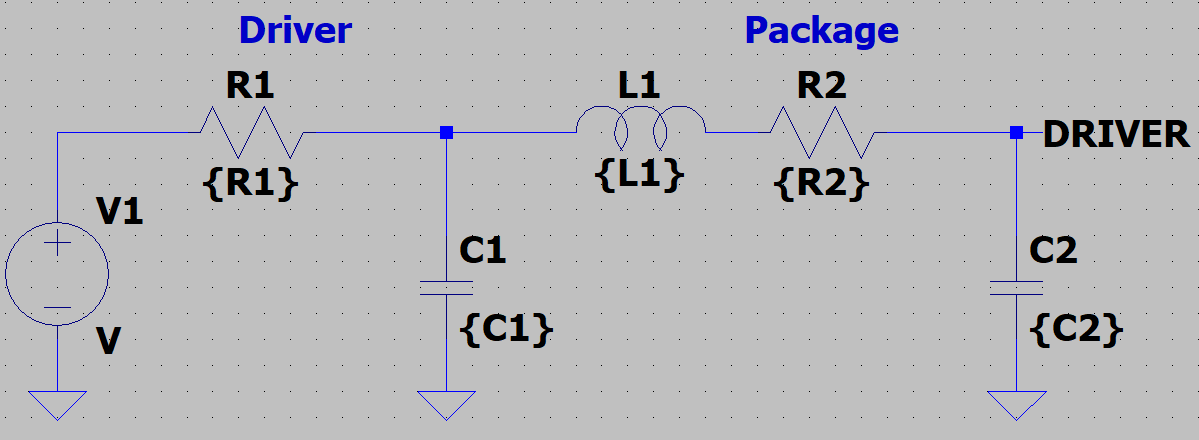
\includegraphics[width=0.8\textwidth]{ltspice_driver.png}}
    \caption{74ALVC244 driver and package model (QFN).}
    \label{fig:driver-package}
\end{figure}

\newpage

\subsubsection{Buffer Input Model}

Consider the generic input buffer shown in Figure \ref{fig:ibis-input}. Again we have $C_{pkg}, R_{pkg}, L_{pkg}$ to model the package parasitics. Since the signal will drive the gate(s) of a CMOS circuit, it can be modelled as a single capacitor $C_{comp}$.\footcite{ibis}

\begin{figure}[h]
    \centering
    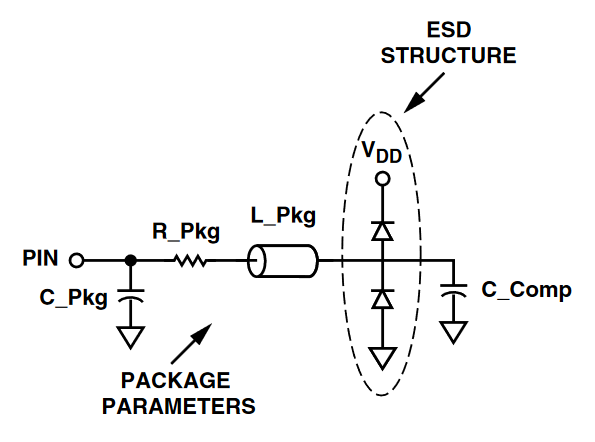
\includegraphics[width=0.5\textwidth]{input-ibis.png}
    \caption{Input buffer\footcite{ibis}.}
    \label{fig:ibis-input}
\end{figure}

The linear model of the receiver circuit is shown in Figure \ref{fig:receiver-package}. $C_4$ describes the receiver and $C_3, L_2, R_7$ model the package.

\begin{figure}[h]
    \centering
    \fbox{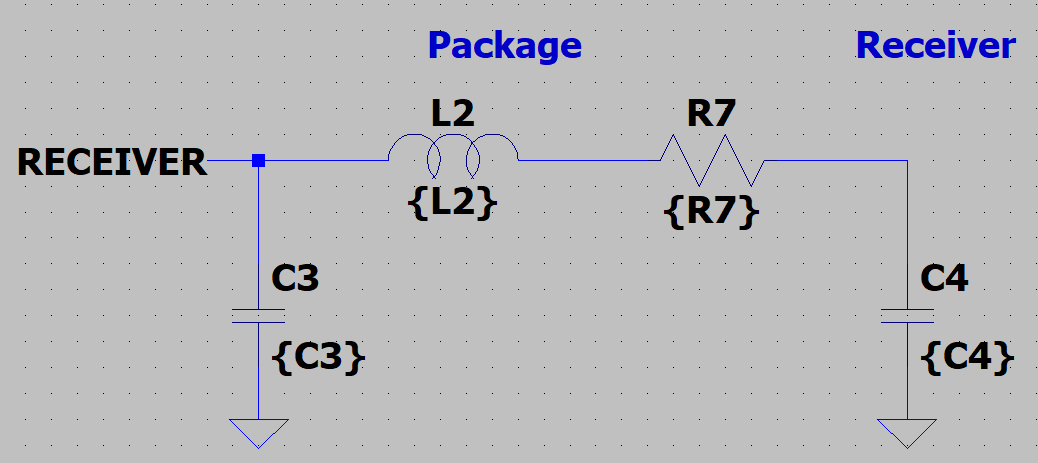
\includegraphics[width=0.8\textwidth]{ltspice_receiver.png}}
    \caption{74ALVC244 receiver and package model (QFN).}
    \label{fig:receiver-package}
\end{figure}

\subsubsection{Transmission Line Model}

To model the transmission lines we will use a \textit{lossless lumped element model}, essentially a series of resistors, capacitors, and inductors. The minimum number of segments to accurately model a transmission line is given by (\ref{eq:seg_min}).

\begin{equation} \label{eq:seg_min}
    N_{seg, min} = 10 \frac{TD}{T_{r}}
\end{equation}

Where $TD$ is the delay of the transmission line, and $T_{r}$ is the rise time of the signal. The time delay, TD, is given by (\ref{eq:td}).

\begin{equation} \label{eq:td}
    TD = \sqrt{L_{total} * C_{total}}
\end{equation}

Denoting the transmission line length $x$, we have the following values for all 3 cases:

\begin{align*}
    x &= 0.01\,\si{m} \\
    T_r &= 500\,\si{ps}
\end{align*}

\newpage

\begin{table}[t]
    \centering
    \begin{tabular}{l|l l}
        \toprule[1pt]
        \textbf{Case} & \textbf{Inductance Matrix} & \textbf{Capacitance Matrix} \\
        \midrule
        Side-by-side microstrip &
        $L_{mat,1} =
        \begin{bmatrix}
            283.4 & 52.2 \\
            52.2 & 283.4
        \end{bmatrix}$ &
        $C_{mat,1} =
        \begin{bmatrix}
            128.5 & -12.0 \\
            -12.0 & 128.5
        \end{bmatrix}$ \\
        && \\
        Side-by-side stripline &
        $L_{mat,2} =
        \begin{bmatrix}
            318.5 & 45.3 \\
            45.3 & 318.5
        \end{bmatrix}$ &
        $C_{mat,2} =
        \begin{bmatrix}
            153.3 & -21.8 \\
            -21.8 & 153.3
        \end{bmatrix}$ \\
        && \\
        Broadside stripline &
        $L_{mat,3} =
        \begin{bmatrix}
            318.0 & 101.4 \\
            101.4 & 318.0
        \end{bmatrix}$ &
        $C_{mat,3} =
        \begin{bmatrix}
            167.5 & -53.5 \\
            -53.5 &167.53
        \end{bmatrix}$ \\
        \bottomrule[1pt]
    \end{tabular}
    \caption{Inductance and capacitance matrices for the three transmission line cases.}
    \label{tab:lc-matrix}
\end{table}

The inductor and capacitor matrices for all three cases are shown in Table \ref{tab:lc-matrix}. The time delay, TD, and thereafter the minimum number of segments, $N_{seg, min}$, are calculated for each case as follows:

\begin{equation*}
    TD_1 = x \sqrt{L_{self} C_{self}} = 0.01\,\si{m} \sqrt{283.4\,\si{nH/m} * 128.5\,\si{pF/m}} = 60.3\,\si{ps}
\end{equation*}
\begin{equation*}
    TD_2 = x \sqrt{L_{self} C_{self}} = 0.01\,\si{m} \sqrt{318.5\,\si{nH/m} * 153.3\,\si{pF/m}} = 69.9\,\si{ps}
\end{equation*}
\begin{equation*}
    TD_3 = x \sqrt{L_{self} C_{self}} = 0.01\,\si{m} \sqrt{318.0\,\si{nH/m} * 167.5\,\si{pF/m}} = 73.0\,\si{ps}
\end{equation*}
\begin{equation*}
    N_{seg,1} = 10 \frac{TD_1}{T_r} = 10 \frac{60.3\,\si{ps}}{500\,\si{ps}} = 1.21 \approx 2
\end{equation*}
\begin{equation*}
    N_{seg,2} = 10 \frac{TD_2}{T_r} = 10 \frac{69.9\,\si{ps}}{500\,\si{ps}} = 1.40 \approx 2
\end{equation*}
\begin{equation*}
    N_{seg,3} = 10 \frac{TD_3}{T_r} = 10 \frac{73.0\,\si{ps}}{500\,\si{ps}} = 1.46 \approx 2
\end{equation*}

We see that all cases \textit{luckily} only require 2 segments. The lumped element model for the transmission lines is shown in Figure \ref{fig:transmission-line}. Inductors $L_{11}, L_{21}$ and $L_{12}, L_{22}$ are coupled, and capacitors $C_{m}, C_{m2}$ are the mutual capacitances. Together they model the crosstalk between the lines. Resistors $R_3, R_4, R_5, R_6, R_8$ are physical SMD resistors on the PCB.

\begin{figure}[h]
    \centering
    \fbox{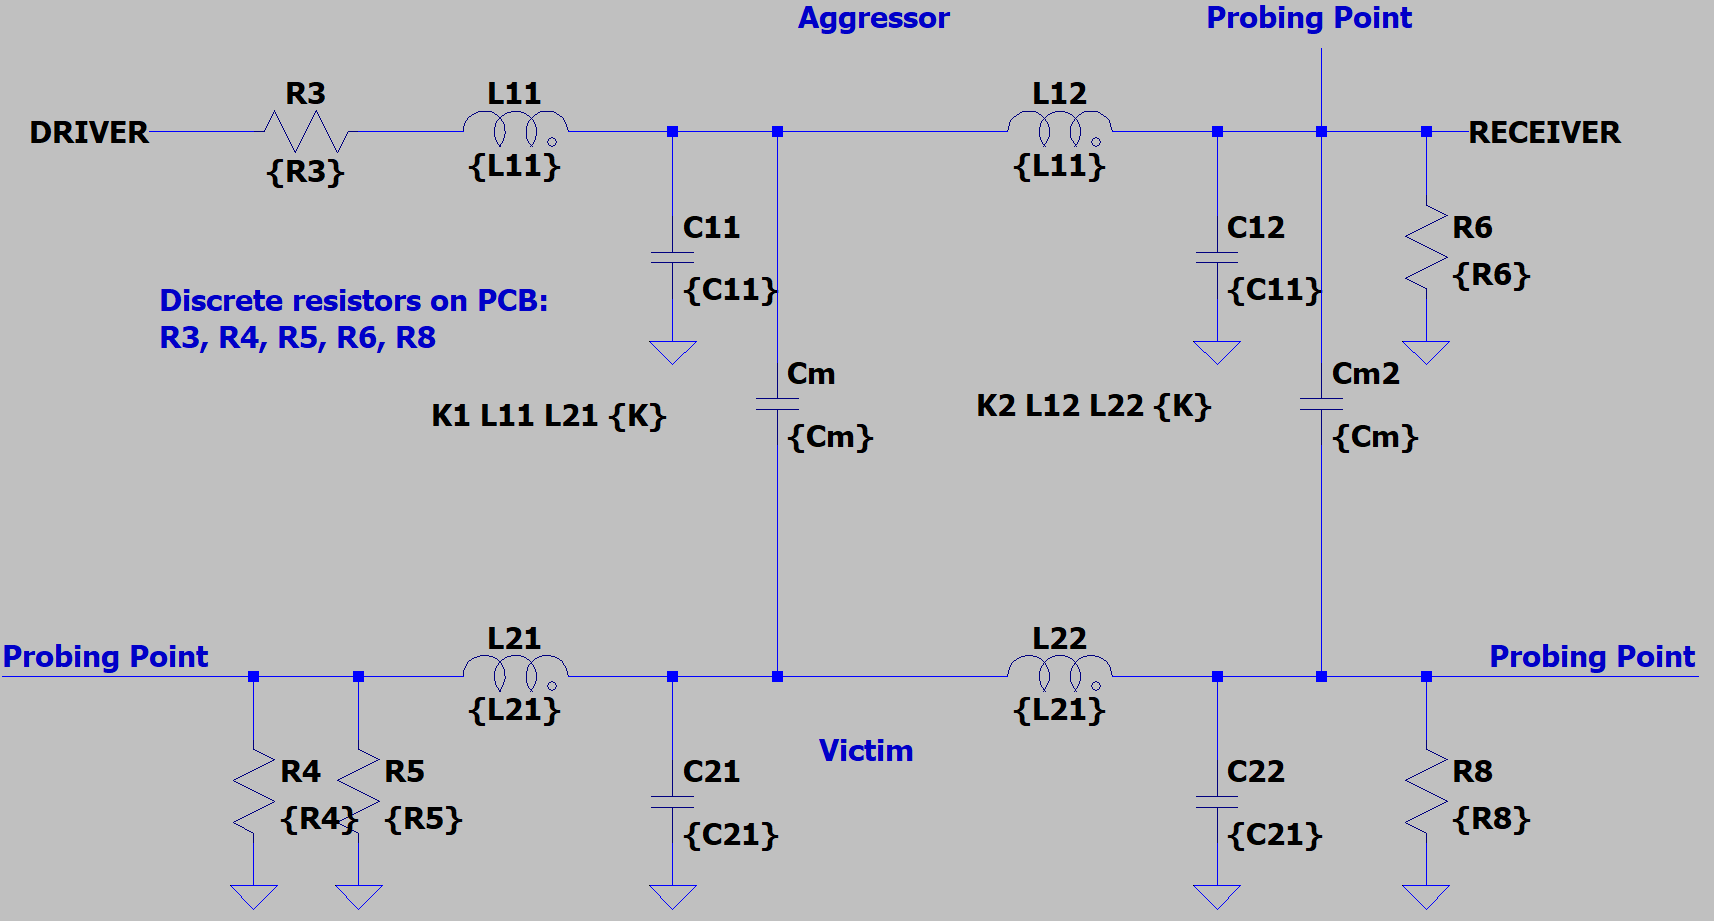
\includegraphics[width=0.8\textwidth]{ltspice_tl.png}}
    \caption{Lumped element model for the transmission lines.}
    \label{fig:transmission-line}
\end{figure}

\newpage

\subsection{Task 1.2}

Find and estimate the values of the different parameters based on data from the HW test-board, PCB schematic, and the datasheet and IBIS model for the driver/receiver IC. Assume that the aggressor line is matched at the driver end.

\solution

\subsubsection{Output Buffer Model Parameters}

Capacitor $C_{comp}$ is found to be $6.04\,\si{pF}$ (typically) in the IBIS model for the 74ALVC244 at a supply voltage of $V_{DD} = 3.3\,\si{V}$. Package parameters depend on which output pins are used and are summarized in Table \ref{tab:pkg-params}.

\begin{table}[h]
    \centering
    \begin{tabular}{l|l l l l}
        \toprule[1pt]
        \textbf{Case} & \textbf{Pin} & $R_{pkg}$ [$\si{\ohm}$] & $C_{pkg}$ [$\si{pF}$] & $L_{pkg}$ [$\si{nH}$] \\
        \midrule
        Side-by-side microstrip & 1Y2 & 0.09336 & 0.15918 & 1.33430 \\
        Side-by-side stripline  & 1Y3 & 0.10013 & 0.14031 & 1.44133 \\
        Broadside stripline     & 1Y4 & 0.11819 & 0.15918 & 1.73153 \\
        \bottomrule[1pt]
    \end{tabular}
    \caption{Package parameters for the 74ALVC244 buffer (QFN).}
    \label{tab:pkg-params}
\end{table}

It is assumed that $R_1 = 10.9\,\si{\Omega}$, even though it varies depending on if it "pulls" up or down.

\subsection{Task 1.3}

For each of the transmission lines calculate the equivalent circuit model of the system of the coupled transmission lines. Assume $T_{rise} = 500\,\si{ps}$.

\solution

\subsection{Task 1.4}

From the datasheet - what are the minimum high input and output levels and the maximum low input and output levels. (Assume $V_{CC} = 3.3\,\si{V} \pm 5\%$, and use the same max current load $\pm 12 \,\si{mA}$ for both output low and high).

\solution

\subsection{Task 1.5}

Simulate for each of the transmission line configurations the circuit model (Driver 0-3.3V, $T_{rise} = 500\,\si{ps}$).

\vspace{10pt}
Document the voltage curves over time, at the driver and receiver ends of the aggressor line, and the near-end (NEXT) and far-end (FEXT) crosstalk at the victim line.

\vspace{10pt}
Determine the critical crosstalk level in the low state and (high) state. The critical crosstalk level when the line is in a low (high) state is the maximum (minimum) voltage over the victim line due to crosstalk.

\solution

\end{document}
